\section*{سوال ۵}

در این بخش، پنج مفهوم مدل‌سازی عمده در مهندسی نرم‌افزار -
\lr{DFD}
،
\lr{UML}
،
\lr{User Story}
،
\lr{CRC Card}
و
\lr{BPMN}
- مورد بررسی و مقایسه قرار دهید از جنبه‌های مختلف.

\begin{itemize}
	\item چه چیزهایی را مدل می‌کنند
	\item آن‌ها را چگونه مدل می‌کنند
	\item کجا/در چه زمانی استفاده می‌شوند
	\item تفاوت سطح انتزاع در مدل‌سازی
\end{itemize}

\section*{جواب سوال ۵}

در مهندسی نرم‌افزار، مدل‌سازی فرایندی است که به منظور ایجاد یک نمایش گرافیکی یا نمادین از یک سیستم، فرایند یا مفهوم انجام می‌شود. مدل‌سازی می‌تواند برای اهداف مختلفی استفاده شود، از جمله:

تجسم سیستم یا فرآیند

درک بهتر سیستم یا فرآیند

ارتباط موثرتر با سایرین در مورد سیستم یا فرآیند

تجزیه و تحلیل و بهبود سیستم یا فرآیند

در این مقاله، مفاهیم مختلف مدل‌سازی در مهندسی نرم‌افزار را تحلیل و مقایسه می‌کنیم.

BPMN مخفف Business Process Model and Notation به معنای مدل و نشانه‌گذاری فرآیند کسب‌وکار است. این یک زبان مدل‌سازی بصری برای برنامه‌های تجزیه و تحلیل کسب‌وکار و مشخص کردن گردش کار فرایندهای سازمانی است. BPMN توسط ابتکار مدیریت فرآیند کسب‌وکار (BPMI) توسعه یافت و از زمان ادغام دو سازمان در سال ۲۰۰۵ توسط گروه مدیریت اشیاء (OMG) حفظ شده‌است.

\subsubsection*{عناصر اصلی}

BPMN از مجموعه‌ای از عناصر بصری برای مدل‌سازی فرآیندهای کسب‌وکار استفاده می‌کند. این عناصر عبارتند از:

\begin{itemize}
	\item فعالیت‌ها (Activities): فعالیت‌ها اقداماتی هستند که در یک فرآیند انجام می‌شوند. فعالیت‌ها می‌توانند شامل کارهای فیزیکی، پردازش اطلاعات یا تصمیم‌گیری باشند.
	\item جریان‌ها (Flows): جریان‌ها نحوه ارتباط فعالیت‌ها را نشان می‌دهند. جریان‌ها می‌توانند به صورت خط مستقیم، خط نقطه‌چین یا خط مورب نشان داده شوند.
	\item شروع و پایان (Start and End): شروع و پایان نشان‌دهنده نقاط شروع و پایان یک فرآیند هستند.
	\item کنترل‌ها (Controls): کنترل‌ها شرایطی را که بر جریان فرآیند تأثیر می‌گذارند، نشان می‌دهند.
	\item پیوندها (Links): پیوندها فعالیت‌ها یا جریان‌های مختلف را به هم متصل می‌کنند.
\end{itemize}

\subsubsection*{مزایای استفاده از BPMN}

BPMN مزایای متعددی برای سازمان‌ها دارد، از جمله:

\begin{itemize}
	\item **توضیح واضح فرآیندهای کسب‌وکار:** BPMN یک زبان بصری است که به مدیران و ذینفعان کسب‌وکار کمک می‌کند تا فرآیندهای کسب‌وکار را به‌طور واضح و مختصر درک کنند.
	\item **بهبود ارتباط بین ذینفعان:** BPMN به مدیران و ذینفعان کسب‌وکار کمک می‌کند تا در مورد فرآیندهای کسب‌وکار به‌طور موثرتر ارتباط برقرار کنند.
	\item **افزایش کارایی و بهره‌وری:** BPMN می‌تواند به سازمان‌ها کمک کند تا فرآیندهای کسب‌وکار خود را بهبود بخشند و کارایی و بهره‌وری را افزایش دهند.
	\item **کاهش ریسک:** BPMN می‌تواند به سازمان‌ها کمک کند تا ریسک‌های مرتبط با فرآیندهای کسب‌وکار خود را کاهش دهند.
\end{itemize}

\subsubsection*{کاربردهای BPMN}

BPMN در طیف گسترده‌ای از کاربردها استفاده می‌شود، از جمله:

\begin{itemize}
	\item **تجزیه و تحلیل فرآیندهای کسب‌وکار:** BPMN می‌تواند برای تجزیه و تحلیل فرآیندهای کسب‌وکار موجود و شناسایی فرصت‌های بهبود استفاده شود.
	\item **طراحی فرآیندهای کسب‌وکار جدید:** BPMN می‌تواند برای طراحی فرآیندهای کسب‌وکار جدید استفاده شود.
	\item **پیاده‌سازی فرآیندهای کسب‌وکار:** BPMN می‌تواند برای پیاده‌سازی فرآیندهای کسب‌وکار در سیستم‌های فناوری اطلاعات استفاده شود.
	\item **آموزش فرآیندهای کسب‌وکار:** BPMN می‌تواند برای آموزش کارکنان در مورد فرآیندهای کسب‌وکار استفاده شود.
\end{itemize}

\subsubsection*{آینده BPMN}

BPMN یک زبان قدرتمند و انعطاف‌پذیر است که به سازمان‌ها کمک می‌کند تا فرآیندهای کسب‌وکار خود را به‌طور موثرتر مدیریت کنند. انتظار می‌رود که BPMN در سال‌های آینده به محبوبیت خود ادامه دهد، زیرا سازمان‌ها به دنبال راه‌هایی برای بهبود کارایی و بهره‌وری خود هستند.


\begin{figure}[H]
	\centering
	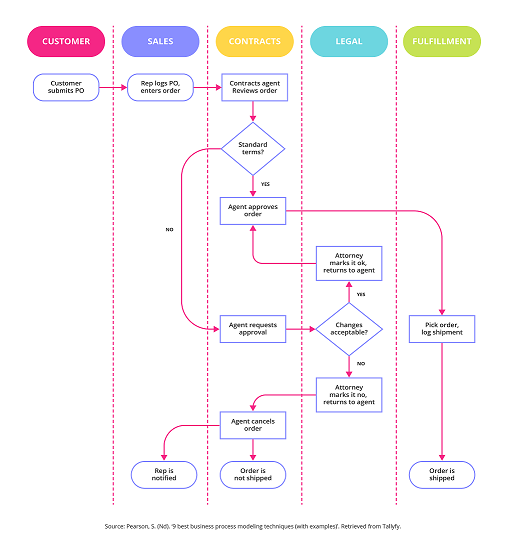
\includegraphics{pic5.png}
	\label{fig:label4}
\end{figure}

\section*{\lr{DFD (Data Flow Diagram)}}
\begin{itemize}
	\item \textbf{چه چیزهایی را مدل می‌کند:} جریان داده‌ها و ارتباطات بین فرایندها، داده‌ها و ذخیره‌سازی‌ها.
	\item \textbf{چگونگی مدل‌سازی:} با استفاده از نمودارهای گرافیکی برای نشان دادن جریان داده‌ها.
	\item \textbf{زمان استفاده:} در مراحل اولیه تحلیل سیستم برای درک بهتر جریان اطلاعات.
	\item \textbf{سطح انتزاع:} سطح بالا در ارتباط با جریان داده‌ها.
\end{itemize}

\section*{\lr{UML (Unified Modeling Language)}}
\begin{itemize}
	\item \textbf{چه چیزهایی را مدل می‌کند:} ساختار و رفتار سیستم‌های نرم‌افزاری.
	\item \textbf{چگونگی مدل‌سازی:} با استفاده از مجموعه‌ای متنوع از نمودارها (مانند نمودار کلاس، نمودار توالی).
	\item \textbf{زمان استفاده:} در تمام مراحل توسعه نرم‌افزار.
	\item \textbf{سطح انتزاع:} متغیر، بسته به نوع نمودار.
\end{itemize}

\section*{\lr{User Story}}
\begin{itemize}
	\item \textbf{چه چیزهایی را مدل می‌کند:} نیازمندی‌ها و ویژگی‌های کاربران از دیدگاه آن‌ها.
	\item \textbf{چگونگی مدل‌سازی:} به صورت جملات ساده و قابل فهم برای توصیف داستان‌های کاربری.
	\item \textbf{زمان استفاده:} بیشتر در رویکردهای توسعه چابک.
	\item \textbf{سطح انتزاع:} بسیار بالا و کاربر محور.
\end{itemize}

\section*{\lr{CRC Card (Class-Responsibility-Collaboration)}}
\begin{itemize}
	\item \textbf{چه چیزهایی را مدل می‌کند:} وظایف، مسئولیت‌ها و همکاری‌های کلاس‌ها.
	\item \textbf{چگونگی مدل‌سازی:} با استفاده از کارت‌هایی که کلاس‌ها و وظایف آن‌ها را نمایش می‌دهند.
	\item \textbf{زمان استفاده:} در مرحله طراحی سیستم و تعریف مسئولیت‌های کلاس‌ها.
	\item \textbf{سطح انتزاع:} متوسط تا بالا در ارتباط با ساختار کلاس‌ها.
\end{itemize}

\section*{\lr{BPMN (Business Process Model and Notation)}}
\begin{itemize}
	\item \textbf{چه چیزهایی را مدل می‌کند:} فرایندهای کسب‌وکار و وظایف مرتبط.
	\item \textbf{چگونگی مدل‌سازی:} با استفاده از نمودارهای فرایندی و نشانه‌گذاری‌های استاندارد.
	\item \textbf{زمان استفاده:} برای تحلیل و بهبود فرایندهای کسب‌وکار.
	\item \textbf{سطح انتزاع:} بالا در ارتباط با فرایندهای سازمانی.
\end{itemize}


